% This is a template for creating lecture notes using Chirun. It includes commonly used packages and settings. You can modify it as needed.

\documentclass{article} % This is the document class. Article is the most common class for single-page lecture notes. If you want your entire module's notes in one Chirun document, use report or book instead. 
\usepackage{booktabs} % This package is used for creating tables
\usepackage[colorlinks,linkcolor={blue}]{hyperref} % This package is used for hyperlinks
\usepackage[dvipsnames]{xcolor} % This package is used for colors e.g. shaded boxes
\usepackage{chirun} % This package is used for adding \alttext, embedding videos, numbas packages, etc.
\usepackage{amsfonts, amsmath, amssymb, amsthm} % These packages are used for mathematical symbols
\usepackage{graphicx} % This package is used for adding images
\usepackage{listings} % This package is used for code highlighting
\usepackage[most]{tcolorbox} % This package is used for creating colored boxes
\usepackage[authoryear]{natbib} % This package is used for citations
\bibliographystyle{agsm} % This is the bibliography style. You can change it.
\usepackage{pgfplots} % This package is used for creating plots.
\pgfplotsset{width=10cm,compat=1.9} % This sets the default width of plots and the compatibility level.
\usepackage{tikz} % This package is used for creating diagrams.
\usepackage{xspace} % This package is used for spacing after macros.

% The following lines define styles for TikZ diagrams.
\tikzset{
  startstop/.style={rectangle, rounded corners, minimum width=3cm, minimum height=1cm,text centered, draw=black, fill=gray!20},
  decision/.style={diamond, aspect=2, minimum width=3.5cm, minimum height=1cm, text centered, draw=black, fill=blue!20},
  process/.style={rectangle, minimum width=3.5cm, minimum height=1cm, text centered, draw=black, fill=green!20},
  arrow/.style={thick, ->, >=stealth}
}

% The following lines set the page margins and paragraph spacing.
\setlength{\parindent}{0pt}
\setlength{\parskip}{1em}

% New colors defined below
\definecolor{codegreen}{rgb}{0,0.6,0}
\definecolor{codegray}{rgb}{0.5,0.5,0.5}
\definecolor{codepurple}{rgb}{0.58,0,0.82}
\definecolor{backcolour}{rgb}{0.95,0.95,0.92}

% Simple code listing style that works reliably in Chirun
\lstdefinestyle{mystyle}{
  backgroundcolor=\color{backcolour},   
  basicstyle=\ttfamily\footnotesize,
  breakatwhitespace=false,         
  breaklines=true,                 
  captionpos=b,                    
  keepspaces=true,                 
  numbers=left,                    
  numbersep=5pt,                  
  showspaces=false,                
  showstringspaces=false,
  showtabs=false,                  
  tabsize=2,
  frame=single,
  rulecolor=\color{codegray}
}

% "mystyle" code listing set
\lstset{style=mystyle}

\title{LaTeX starter template for Chirun} % This is the title of your document.
\author{Ross Parker}

\begin{document}

\maketitle

\section{What is this template for?} % This is a section heading. Think of this as a Heading 1 in Word.
This document serves as a LaTeX template for anyone new to using Chirun. It contains LaTeX packages that have been tested and we know are supported by Chirun. It includes examples of commonly used features such as sections, images, quotations, lists, math equations, tables, colored boxes, code highlighting, videos, and scientific charts and diagrams. You can modify it as needed.

\subsection{How should I use this template?} % This is a subsection heading. Think of this as a Heading 2 in Word.
The document serves as a starting point for creating your own lecture notes using Chirun. The intention is to replace the placeholder text \textit{like this}  with your own document. You can delete or comment out any sections you don't need. For more information on using Chirun, visit the \href{https://chirun.org.uk/docs/en/latest/}{Chirun documentation} \citep{chirunTutorial}.

Here's a suggested workflow:

\begin{enumerate}
    \item \textbf{Download} – Download a copy of this file.
    \item \textbf{Open it in a LaTeX editor} – Open the file in a LaTeX editor of your choice. I use VS Code with LaTeX extensions, but you may prefer to use Overleaf or something you're more familiar with
    \item \textbf{Copy and paste} – Copy and paste content from your own LaTeX notes into this template, replacing the placeholder text I've added. Remember to save your work regularly.
    \item \textbf{Upload} – Upload your file to Chirun \href{https://lti.chirun.org.uk/}{Chirun LTI Tool} to convert it to HTML. If you have multiple files, you can zip them into a single archive and upload that instead.
\end{enumerate}

\section{How do I add images in Chirun?} % This is another section heading.

Adding images - or \textit{figures} - as they're referred to in LaTeX makes use of the \verb|\chirun| package. This package allows you to add alternative text to images using the \verb|\alttext| command. If you use assistive technologies such as a screenreader, the image below will be read out as: \textbf{'A snail with a yellow and brown spiral patterned shell on the top of a red mushroom.'} Without the \verb|\alttext| command, the screenreader would read out the file name of the image instead, which is not very helpful and could unfairly disadvantage anyone with a visual impairment.

\begin{figure}
   \includegraphics[width=0.8\textwidth]{images/snail.jpg}
    \caption{A spiral formed by Fibonacci-numbered squares resembles a snail shell—an elegant pattern often used in art and design. Photo by \href{https://unsplash.com/@epan5?utm_content=creditCopyText&utm_medium=referral&utm_source=unsplash}{Krzysztof Niewolnyn} on \href{https://unsplash.com/photos/brown-snail-on-red-mushroom-during-daytime-q6wb__wgnew}{Unsplash}}
    \alttext{A snail with a yellow and brown spiral patterned shell on the top of a red mushroom.}
\end{figure}

\section{How does Chirun handle equations?}
When converting LaTeX documents to HTML usign Chirun, mathematical notation is rendered using \href{https://www.mathjax.org/}{MathJax}. This ensures that equations are displayed clearly in web browsers and remain accessible to screen readers and other assistive technologies.

\subsection{Closed-form Formula (Binet's Formula)}

We can also calculate the $n$th Fibonacci number directly using a closed-form formula, though it's a bit more complex:

\begin{equation}
F_n = \frac{1}{\sqrt{5}} \left( \phi^n - \left( -\frac{1}{\phi} \right)^n \right)
\end{equation}

where $\phi$ (phi) is the golden ratio:

\begin{equation}
\phi = \frac{1 + \sqrt{5}}{2}
\end{equation}

\subsection{The Golden Ratio}

As the sequence continues, the ratio between consecutive Fibonacci numbers approaches the golden ratio:

\begin{equation}
\lim_{n \to \infty} \frac{F_{n+1}}{F_n} = \phi \approx 1.618
\end{equation}

This ratio appears in many areas of nature, design, and photography.

\subsection{Matrix Representation}

Fibonacci numbers can even be represented using matrices, which is useful for advanced calculations:

\begin{equation}
\begin{bmatrix}
F_{n+1} \\
F_n
\end{bmatrix}
=
\begin{bmatrix}
1 & 1 \\
1 & 0
\end{bmatrix}^n
\begin{bmatrix}
1 \\
0
\end{bmatrix}
\end{equation}

\begin{quote}
    \textit{``The Fibonacci Sequence turns out to be the key to understanding how nature designs... and is... a part of the same ubiquitous music of the spheres that builds harmony into atoms, molecules, crystals, shells, suns and galaxies and makes the Universe sing.''}

    \smallskip % a little vertical space
    \textbf{Guy Murchie}
\end{quote}

\section{How about tables in Chirun?}
Chirun supports a wide range of common LaTeX packages. When you are writing your document, you can often include them as you normally would. Below is a table showing a few examples of supported packages and their status. For a complete and up-to-date list, you can visit the \href{https://chirun.org.uk/docs/en/latest/reference/latex/supported_packages.html}{full Chirun documentation}.

\begin{table}[h]
    \centering
    \begin{tabular}{l l}
        \toprule
        \textbf{Package Name} & \textbf{Status} \\
        \midrule
        \texttt{amsmath} & Re-implemented by \texttt{plasTeX} \\
        \texttt{booktabs} & Re-implemented by \texttt{plasTeX} \\
        \texttt{caption} & Re-implemented by Chirun \\
        \texttt{enumitem} & Re-implemented by Chirun \\
        \texttt{graphicx} & Re-implemented by \texttt{plasTeX} \\
        \texttt{hyperref} & Re-implemented by \texttt{plasTeX} \\
        \texttt{listings} & Re-implemented by \texttt{plasTeX} \\
        \texttt{longtable} & Re-implemented by \texttt{plasTeX} \\
        \texttt{multirow} & No problems observed \\
        \texttt{natbib} & Re-implemented by \texttt{plasTeX} \\
        \texttt{pgfplots} & Re-implemented by \texttt{plasTeX} \\
        \texttt{pstricks} & Re-implemented by \texttt{plasTeX} \\
        \texttt{siunitx} & Supported (MathJax package) \\
        \texttt{soul} & No problems observed \\
        \texttt{subcaption} & Re-implemented by Chirun \\
        \texttt{tcolorbox} & Re-implemented by Chirun \\
        \texttt{tikz} & Re-implemented by \texttt{plasTeX} \\
        \texttt{todonotes} & Re-implemented by \texttt{plasTeX} \\
        \texttt{ulem} & Re-implemented by Chirun \\
        \texttt{xcolor} & Re-implemented by \texttt{plasTeX} \\
        \bottomrule
    \end{tabular}
    \caption{A selection of supported LaTeX packages in Chirun.}
    \label{tab:chirun_packages}
\end{table}

\section{Does Chirun support colored boxes for things like theorems and examples?}
Shaded boxes are supported using the \verb|tcolorbox| package. The colours can be applied using the \verb|[dvipsnames]| option within the \verb|xcolor| package.

\subsection{A Yellow Box with a Heading Section}
\begin{tcolorbox}[colback=Goldenrod!10,colframe=Goldenrod!60!black,
    colbacktitle=Goldenrod!70!black,title=Tip]
    Chirun isn't limited to standard LaTeX documents. You can also create Beamer presentations, Markdown documents, and Markdown slides that use the Reveal.js framework. You can view examples of these by visiting the \href{https://www.chirun.org.uk/demo/}{Chirun Sample Course}.
\end{tcolorbox}

\section{How does Chirun handle code syntax highlighting?}

Code can be highlighted using the \verb|listings| package. The following example shows how to create a function that computes the incidence matrix of two generators.
The function \verb|incmatrix| takes two lists of generators as input and returns the incidence matrix. The code is written in Python and uses \href{https://numpy.org/}{NumPy} for matrix operations.

\begin{lstlisting}[language=Python, caption=Python example]
import numpy as np
    
def incmatrix(genl1,genl2):
    m = len(genl1)
    n = len(genl2)
    M = None #to become the incidence matrix
    VT = np.zeros((n*m,1), int)  #dummy variable
    
    #compute the bitwise xor matrix
    M1 = bitxormatrix(genl1)
    M2 = np.triu(bitxormatrix(genl2),1) 

    for i in range(m-1):
        for j in range(i+1, m):
            [r,c] = np.where(M2 == M1[i,j])
            for k in range(len(r)):
                VT[(i)*n + r[k]] = 1;
                VT[(i)*n + c[k]] = 1;
                VT[(j)*n + r[k]] = 1;
                VT[(j)*n + c[k]] = 1;
                
                if M is None:
                    M = np.copy(VT)
                else:
                    M = np.concatenate((M, VT), 1)
                
                VT = np.zeros((n*m,1), int)
    
    return M
\end{lstlisting}


\section{The Chirun package allows HTML content}
As we're converting to HTML rather than just PDF we can add in some additional functionality such as video embeds and custom HTML.

\subsection{Embedding Videos}
Videos can be embedded from YouTube or Vimeo so they appear in the HTML output. They are rendered as hyperlinks in the PDF output. For more information visit the \href{https://chirun.org.uk/docs/en/latest/reference/latex/chirun_package.html}{Chirun LaTeX package documentation} \citep{chirunTutorial}.
\youtube[YouTube:]{BAIAlWS3FRE}

\subsection{Custom HTML}
\begin{HTML}
<p>The Chirun package allows you to also add custom HTML elements. This can be useful for adding things like interactive content, maps, widgets, or in this case silly emojis 👾 and gifs.</p>

    <iframe src="https://giphy.com/embed/cyMqOH8rjgDHG" width="369" height="480" style="" frameBorder="0" class="giphy-embed" allowFullScreen></iframe><p><a href="https://giphy.com/gifs/pac-man-cyMqOH8rjgDHG">Gif of Pacman 80's arcade game via GIPHY</a></p>
\end{HTML}

\section{What about scientific charts and diagrams?}
For plotting mathematical expressions and creating diagrams, Chirun supports the \verb|pgfplots| and \verb|tikz| packages. Below are some examples of how to create line graphs and 3D surface plots.

\subsection{Plotting Mathematical Expressions Using a Line Graph}
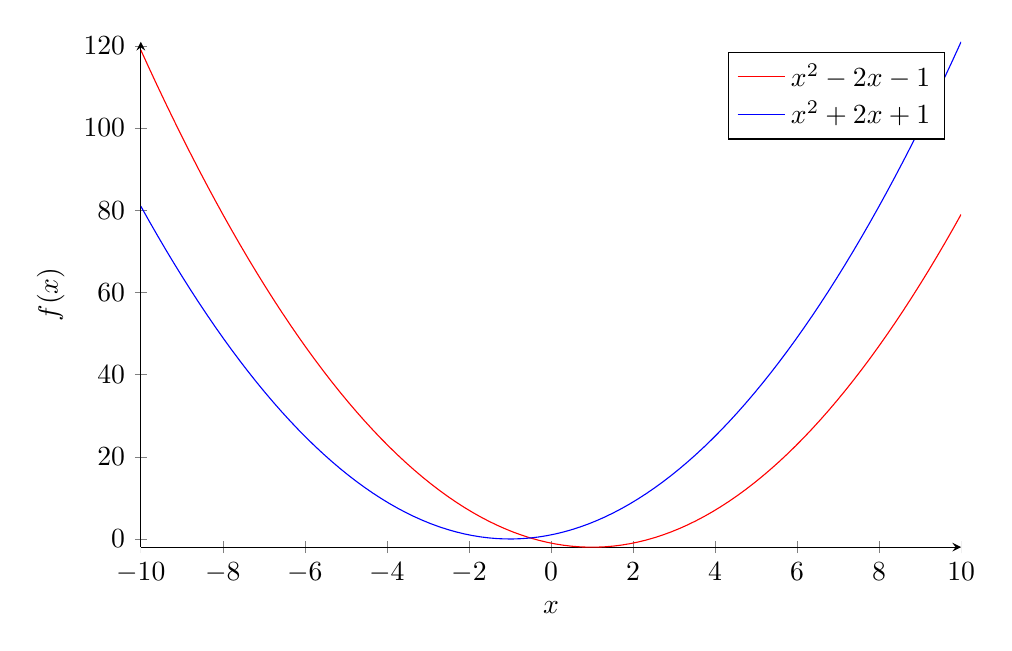
\begin{tikzpicture}
\begin{axis}[
    width=12cm, height=8cm, % Increased size
    axis lines = left,
    xlabel = \(x\),
    ylabel = {\(f(x)\)},
]
% Below the red parabola is defined
\addplot [
    domain=-10:10, 
    samples=100, 
    color=red,
]
{x^2 - 2*x - 1};
\addlegendentry{\(x^2 - 2x - 1\)}

% Here the blue parabola is defined
\addplot [
    domain=-10:10, 
    samples=100, 
    color=blue,
]
{x^2 + 2*x + 1};
\addlegendentry{\(x^2 + 2x + 1\)}
\end{axis}
\end{tikzpicture}

\subsection{Plotting Mathematical Expressions Using the Mesh Parameter}
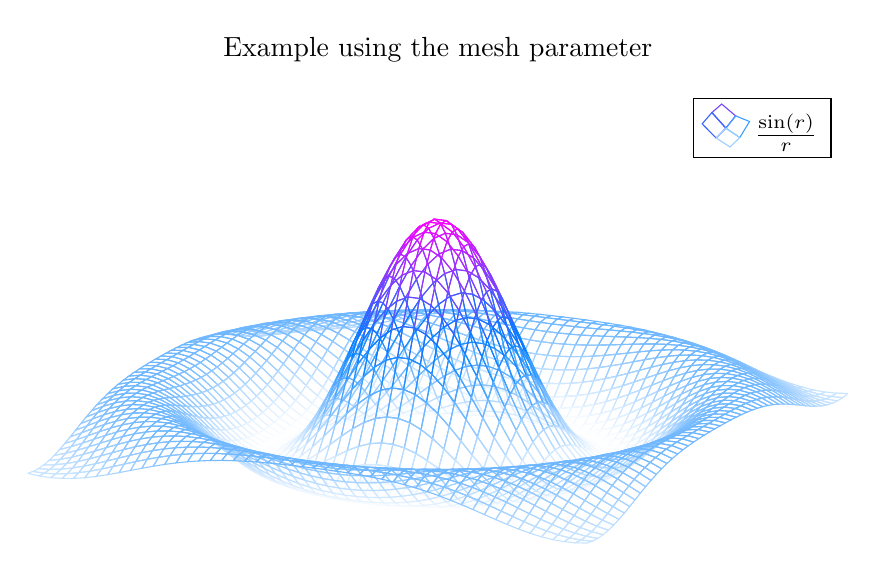
\begin{tikzpicture}
\begin{axis}[
    width=12cm, height=8cm, % Increased size
    title=Example using the mesh parameter,
    hide axis,
    colormap/cool,
]
\addplot3[
    mesh,
    samples=50,
    domain=-8:8,
]
{sin(deg(sqrt(x^2+y^2)))/sqrt(x^2+y^2)};
\addlegendentry{\(\frac{\sin(r)}{r}\)}
\end{axis}
\end{tikzpicture}

\bibliography{references}

\end{document}